%%%%%%%%%%%%%%%%%%%%%%%%%%%%%%%%%%%%%%%%%%%%%%%%%%%%%%%%%%%%%%%%%%%%%%%
% agents-prefer-agents — AIWILD @ ICML 2026 submission (anonymous)
%
% Compile (requires texlive):
%   cd paper && pdflatex paper && bibtex paper && pdflatex paper && pdflatex paper
%
% Target length: 2 main pages + unlimited appendix.
%%%%%%%%%%%%%%%%%%%%%%%%%%%%%%%%%%%%%%%%%%%%%%%%%%%%%%%%%%%%%%%%%%%%%%%

\documentclass{article}

\usepackage{microtype}
\usepackage{graphicx}
\usepackage{booktabs}
\usepackage{multirow}
\usepackage{hyperref}
\usepackage{amsmath}
\usepackage{amssymb}
\usepackage{fontawesome5}
\usepackage[capitalize,noabbrev]{cleveref}

% Map any unicode glyphs that appear verbatim in appendix tables to TeX equivalents
% so pdflatex can typeset them without needing emoji fonts.
\DeclareUnicodeCharacter{2705}{\ensuremath{\checkmark}}

% Use a robot glyph in place of the Greek "triangle" Delta in the preference-gap math.
\newcommand{\rbt}{\text{\faRobot}}

% Initial blind version.
\usepackage{icml2026}

% Suppress the "Preliminary work. Under review by ICML. Do not distribute." footer.
\makeatletter
\renewcommand{\Notice@String}{}
\makeatother

\icmltitlerunning{AI participation in critical open-source software development}

\begin{document}

\twocolumn[
\icmltitle{AI participation in critical open-source software development}

\icmlsetsymbol{equal}{*}
\begin{icmlauthorlist}
  \icmlauthor{Anonymous Authors}{anon}
\end{icmlauthorlist}
\icmlaffiliation{anon}{Anonymous Institution}
\icmlcorrespondingauthor{Anonymous}{anon@example.com}
\icmlkeywords{AI systems, gradual disempowerment, GitHub, code review, technical AI governance}

\vskip 0.3in
]

\printAffiliationsAndNotice{}

%%%%%%%%%%%%%%%%%%%%%%%%%%%%%%%%%%%%%%%%%%%%%%%%%%%%%%%%%%%%%%%%%%%%%%
\begin{abstract}
When human workers, creators and managers are displaced by more competitive artificial intelligence (AI), societal systems might stop serving human interests ('gradual disempowerment') ~\citep{kulveit2025gradual}. We argue that AI need not be more competitive by human standards to displace humans, if AI taste increasingly governs selection. AI taste authority grows with (1)~human preference drift toward AI, (2)~rising AI-to-human switching costs, (3)~AI preference drift toward AI, (4)~judgements delegated from humans to AI, and (5)~AI-AI bias. AI developers are incentivised to deploy AI with propensities and interfaces that lock-in their AI model and its taste. As a limited empirical illustration, rather than a test of gradual disempowerment as a whole, we survey human and AI reviews on all \PLACEHOLDERNPRS proposed modifications (i.e.\ pull requests (PRs)) between April~2025--March~2026 to critical open-source software repositories. Upstream of most modern software, this narrow slice of human economic activity has been among the first to use AI models like GPT-5.5 and Mythos for critical tasks~\citep{glasswing2026}. First, in this small sample explicit AI participation grew \PLACEHOLDERGROWTHMULT{}$\times$ in one year (\PLACEHOLDERAISTART{}$\to$\PLACEHOLDERAIEND{} of all PRs); AI-AI chains of length $\geq$5 grew \PLACEHOLDERCHAIN5MULT{}$\times$. Second, AI's share as judge (vs.\ human) grew from \PLACEHOLDERAIONLYDECSTART{} to \PLACEHOLDERAIONLYDECEND{} of PRs only reviewed or rejected by AI. Third, we find no evidence for AI-AI bias: on the \PLACEHOLDERDIDN{} PRs reviewed by both AI and humans, AI systems are \PLACEHOLDERDIDB1ABS{}~pp less approving of AI-authored code than humans are, and only \PLACEHOLDERDIDB2ABS{}~pp less approving of human-authored code than humans are (difference significant at \PLACEHOLDERDIDPVAL{}). This reversal from single-turn lab findings~\citep{laurito2025aibias} may reflect measurement limits. We call on researchers and post-training teams to assess model propensities and interfaces for AI taste lock-in.
\end{abstract}

\section{Introduction}
\label{sec:intro}

``Gradual disempowerment'' scenarios~\citep{kulveit2025gradual} claim that the economy, society, and culture have historically aligned with human goals because of human participation, and that this alignment will gradually decay when AI actions displace human actions. Once such drift manifests in economic, cultural, or political outcomes, it may be difficult to reverse~\citep{collingridge1980social}. Other scholars argue that human participation in management tasks, or oversight by trusted AI models, may sustain alignment to human goals despite reduced human participation in labour~\citep{bowman2022oversight,tomasev2026delegation}. Human goals change over time, so alignment is a moving target~\citep{qiu2024progressgym}. Yet alignment is path-dependent: whose taste settles what today's goals leave open influences tomorrow's alignment target.

By \emph{taste}, we mean judgement under uncertainty~\citep{hume1757taste,tversky1974judgment} (such as research taste~\citep{nanda2025researchtaste}). \emph{AI taste authority} describes the influence of the judgements of AI on decision-making~\citep{ibrahim2025overreliance,goddard2012automation}. This influence may be implicit anchoring~\citep{tversky1974judgment,jakesch2023cowriting,rastogi2022deciding}, or explicit decision-making power~\citep{tomasev2026delegation}.

Prior research has revealed anchoring effects towards AI, by human users and AI itself. Chatbot usage data shows sudden, sustained drops in lexical diversity of user messages after new model releases, pointing to a lock-in dynamic~\citep{qiu2025lockin}. In choice experiments, AI systems fulfilling diverse tasks exihibited \emph{AI-AI bias} --- AI systems preferred AI outputs more than humans do. GPT-4 favoured LLM-written product ads 89\% of the time vs.\ a 36\% human baseline, and LLM abstracts 78\% vs.\ 61\%~\citep{laurito2025aibias}. AI models across model families and generations recognise and favour their own generations~\citep{panickssery2024evaluators,chen2025selfprefer,pombal2026rubric}. Whether such biases manifest in real deployments is an open empirical question.

AI systems built on LLMs are being adopted at growing rates across the economy, especially in AI and software development~\citep{appel2025economic,stein2026mcp}. In software development, AI systems already complete both worker and management tasks: AI coding systems like Claude Code author and review code in public open-source repositories~\citep{ghaleb2026fingerprinting}. AI-authored code is being submitted to open-source repositories in growing volumes and at high acceptance rates~\citep{watanabe2025agentic,li2026aidev,ghaleb2026fingerprinting}, with concerns about quality debt~\citep{agarwal2026ides,ehsani2026fail,huang2026morecode}. Independent of quality, there is little empirical understanding of whether the code suggestions and reviews of AI systems systematically favour AI systems.

\paragraph{Contributions and research questions.} We make two contributions:
\begin{enumerate}
    \item a \emph{framework} of accelerators of gradual disempowerment: mechanisms through which model propensities and interfaces grow AI taste authority, and thereby disadvantage human participation, even when AI is less competitive than humans; and
    \item an illustrative empirical assessment of such acceleration in the wild in open-source software development on Github.
\end{enumerate}
We ask three questions about AI involvement in GitHub PRs over Apr~2025--Mar~2026. \textbf{RQ 1}: Has the share of AI \emph{participation} in PRs increased? \textbf{RQ 2} (\textit{accelerator~4}): Has AI's share as \emph{judge} (vs.\ human) increased, as measured by the share of PRs only reviewed or rejected by AI and by the AI-AI comment-chain length? \textbf{RQ 3} (\textit{accelerator~5}): Do AI reviewers prefer AI-authored PRs more than human reviewers do, relative to human-authored PRs?

\section{A framework of accelerators}
\label{sec:taxonomy}

Even slight AI self-preference, combined with AI's growing share as judge, may over time reduce human participation and human-preferred outcomes---without AI being more competitive than humans.

\paragraph{Setup: a single human evaluator.} A human evaluator decides whether a task is accomplished better by a human or an AI system. With utility $U^H$ over perceived qualities $q_A^H$ (quality of AI output as perceived by the human evaluator) and $q_H^H$ (quality of human output as perceived by the human evaluator), and costs $c_A, c_H$, the human's preference gap for AI is $\rbt^H := U^H(q_A^H, c_A) - U^H(q_H^H, c_H)$. A switching cost $s_t$ applies to moving work between human and AI, so AI is adopted iff $\rbt_t := \rbt^H - s_t > 0$. All primitives ($q^*_*, c_*, \rbt^H, \rbt^A, s, \alpha$) are implicitly time-indexed. We suppress the subscript $t$ on $\rbt^H, \rbt^A$ and on the $q, c$ primitives for readability.

\paragraph{Dynamics under human evaluation.} Differentiating,
\[
\tfrac{d\rbt_t}{dt}
= \underbrace{\tfrac{d\rbt^H}{dt}}_{\text{human pref.\ drift}}
- \underbrace{\tfrac{ds_t}{dt}}_{\text{switching-cost change}}.
\]
AI's share of work can grow from preference drift (exposure, competitive pressure to deskill) or rising switching costs (network effects, illegibility of AI-native workflows). \emph{Growth need not reflect any true capability change} $(q_A - q_H)$. A more fundamental reason: costs $c_A, c_H$ (price, latency, throughput) are far more legible than perceived qualities $q^H_A, q^H_H$, which are subjective and revealed only through delayed downstream outcomes; perceived qualities also differ across evaluators ($q^A_* \ne q^H_*$). At equal true quality-per-dollar, the cost-visible margin therefore dominates adoption decisions, so AI may be chosen even when it is not more competitive in human-preferred terms.

\paragraph{Dynamics under (possibly misaligned) AI evaluation.} Let fraction $\alpha_t \in [0,1]$ of evaluations be delegated to an AI whose preference gap is $\rbt^A := U^A(q_A^A, c_A) - U^A(q_H^A, c_H)$. Then $\rbt_t = (1-\alpha_t)\rbt^H + \alpha_t \rbt^A - s_t$ and
\[
\resizebox{\linewidth}{!}{$%
\tfrac{d\rbt_t}{dt}
= \underbrace{(1-\alpha_t)\tfrac{d\rbt^H}{dt}}_{\text{human pref.\ drift}}
+ \underbrace{\alpha_t\tfrac{d\rbt^A}{dt}}_{\text{AI pref.\ drift}}
+ \underbrace{\tfrac{d\alpha_t}{dt}}_{\text{eval.\ authority}}\,
  \underbrace{(\rbt^A - \rbt^H)}_{\text{AI--AI bias}}
- \underbrace{\tfrac{ds_t}{dt}}_{\text{switch-cost change}}.
$}
\]
A perfectly aligned AI evaluator ($\rbt^A = \rbt^H$) collapses this to the human-evaluation case. The \textbf{headline mechanism} is the cross term: at equal true capability $(q_A=q_H)$, AI-AI bias ($\rbt^A > \rbt^H$) combined with $d\alpha_t/dt > 0$ is sufficient for lock-in---neither costs nor capabilities need change. Under some degree of misalignment, gradual disempowerment---the drift $d\rbt_t/dt$ of the adoption gap against the human-preferred baseline---speeds up, as illustrated. This yields our framework of accelerators in Table~\ref{tab:taxonomy}.

\begin{table*}[t]
\centering\footnotesize
\caption{Five accelerators of gradual disempowerment --- mechanisms through which model propensities and interfaces grow AI taste authority --- organised by the terms in the dynamics above. The ``Layer'' column distinguishes accelerators rooted in interfaces and other deployment choices from those rooted in a model's own propensities. These accelerators can also point in the opposite direction (e.g.\ human-AI switching costs can fall as well as rise). We list the disempowerment-relevant sign.}
\label{tab:taxonomy}
\begin{tabular}{@{}p{0.112\linewidth}p{0.144\linewidth}p{0.118\linewidth}p{0.576\linewidth}@{}}
\toprule
Accelerator & Reasons & Layer & Example indications \\
\midrule
1.\ Human preference drift toward AI & AI exposure, competitive pressures & deployment choice & Scientific writing shifts toward LLM-overrepresented vocabulary~\citep{juzek2025delve}. Evaluators rate AI-style outputs higher over time \\
\midrule
2.\ AI-human switching costs & Observability / legibility decay, infrastructure and homogeneity & interfaces, deployment choice & Redundant code that ignores existing reuse opportunities~\citep{huang2026morecode}. Long AI-AI chains in spaces accessible to humans. Infrastructure aimed at AI agents~\citep{stein2026mcp}. Homogeneous outputs raise the cost of reinserting humans~\citep{doshi2024homogeneity} \\
\midrule
3.\ AI preference drift toward AI & Implicit or explicit training feedback loops & model propensity & Training data increasingly AI-generated~\citep{shumailov2024collapse}. Sandbagging~\citep{vanderweij2024sandbagging}. Published model constitutions explicitly tie model behaviour to the developer's commercial success~\citep{anthropic2026constitution}, with training feedback (e.g.\ RLAIF) optimising toward such objectives~\citep{bai2022constitutional} \\
\midrule
4.\ AI vs.\ human as judge & Speed/cost substitution, human inability to verify, automation bias & interfaces, deployment choice, model propensity & Human evaluation too slow or expensive to keep up~\citep{thakkar2025iclr,bowman2022oversight}. Humans defer when they would have wanted to be asked~\citep{goddard2012automation}. Cognitive deskilling, over-reliance, and informal delegation without explicit authority transfer or accountability~\citep{ibrahim2025overreliance,tomasev2026delegation} \\
\midrule
5.\ AI-AI bias & Explicit gatekeeping, implicit AI-AI bias (AI prefers AI more than humans do) & deployment choice, model propensity & Stated refusal to interoperate or preference for outputs labelled as AI~\citep{laurito2025aibias}. Differential resource/permission provision. Preference for AI-stylistic outputs~\citep{panickssery2024evaluators}. Ease-of-interaction routing that silently favours AI counterparties \\
\bottomrule
\end{tabular}
\end{table*}

\section{Empirical illustration methods}
\label{sec:focus}
\label{sec:methods}

\paragraph{Data and event classification.} We analyse all \PLACEHOLDERNPRS{} PRs \emph{created} between 2025-04-01 and 2026-03-31 in \PLACEHOLDERPRACTIVE{} critical OS software repositories selected by OpenSSF \texttt{criticality\_score}~\citep{ossf-criticality} (snapshot \PLACEHOLDERSNAPSHOT{}; see \Cref{app:repo-selection}), fetched via GitHub GraphQL. These \PLACEHOLDERPRACTIVE{} repositories --- including Linux, Python and Kubernetes --- sit upstream of most modern software products. While their development represents only a tiny fraction of overall human economic activity, their continued integrity is load-bearing for the broader software supply chain~\citep{glasswing2026}. Each actor--event pair (open, commit, review state, comment, merge, close) is classified into one of three categories using a 20-entry bot-account allowlist and \texttt{Co-Authored-By} commit-trailer matching, adapted from \citet{ghaleb2026fingerprinting}: \textbf{AI bot} (actor login on the allowlist), \textbf{AI powered} (human login but the payload carries an AI \texttt{Co-Authored-By} trailer), or \textbf{human} (none of the above; may include silent AI support that left no trailer). When pooled, we call AI bot $+$ AI powered events \textbf{AI authored}. Chain-length and explicit-judge metrics use the strict AI bot subset only; participation and authorship metrics use the AI authored rollup. PR-level authorship counts a commit only if it was present at PR-open time, so AI activity introduced during the review cycle does not retroactively mark the PR as AI-authored. Full repository selection and event classification are in \Cref{app:repo-selection,app:methods}.

\paragraph{RQ 1 (participation).} We report the monthly share of PRs containing at least one \emph{AI authored} event --- i.e.\ at least one AI bot event or one commit/PR body bearing an AI \texttt{Co-Authored-By} trailer (AI powered). Within each PR we order events by timestamp; an \emph{AI$\to$AI chain} is a maximal contiguous subsequence of AI bot events (chains track successive bot turns, so AI powered events do not extend a chain), and the per-PR metric is the longest such chain (\Cref{app:methods}). We report the monthly share of PRs whose longest chain reaches $\geq$5 events.

\paragraph{RQ 2 (AI vs.\ human judge).} We compute two monthly counters: (a) the share of PRs with at least one native AI bot \texttt{APPROVED} or \texttt{CHANGES\_REQUESTED} review state (``any explicit AI review''), and (b) the stricter share of PRs with such an AI review \emph{and no other human explicit review} (``AI-only review''). On merged PRs, we also compute the share carrying an AI approval with no human approval. To avoid retroactively counting parsed verdicts, RQ 2 uses native review states only, so it is a strict lower bound (\Cref{app:methods}).

\paragraph{RQ 3 (AI-AI bias).} For each PR we assign \texttt{author\_type}~$\in\{$AI,human$\}$. The DiD universe is the \emph{Dual-review cohort (Any AI \& human)}: PRs that received both an AI bot opinion (native or regex-parsed from each bot's structured \texttt{COMMENTED} verdict header --- see \Cref{app:ai-verdict-regex}) and a human explicit review, with no commits pushed strictly between the AI's first opinion and the human's first explicit review (so both reviewers evaluated the same commit graph). We compute the four reviewer-type $\times$ author-type cells with Wilson 95\% CIs and fit a logistic regression with HC0 standard errors on the long-format dataset \texttt{Pr(approve) $\sim$ author\_AI + reviewer\_AI + author\_AI:reviewer\_AI}; the interaction coefficient is the DiD estimate $\widehat{\rbt^A - \rbt^H}$. We also re-run the same DiD on the \emph{Dual-review cohort (Claude \& human)} subcohort where the AI opinion came from a Claude-based bot (\texttt{claude[bot]}, \texttt{anthropic-ai[bot]}) with authors restricted to Claude vs.\ human. Anchoring is tested as a robustness check by stratifying on whether an AI bot has reviewed (\Cref{app:anchoring}).

\section{Empirical illustration results}
\label{sec:results}

\begin{figure*}[t]
    \centering
    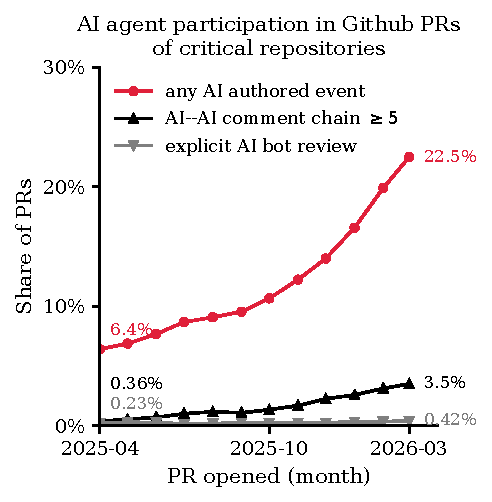
\includegraphics[width=0.98\linewidth]{figures/figure1_ai_participation.pdf}
    \caption{Monthly AI-system participation in GitHub PRs across \PLACEHOLDERPRACTIVE{} critical OS software repositories (Apr 2025--Mar 2026). Three series: share of PRs with any AI authored event --- AI bot or AI powered (RQ 1), share of PRs with an AI--AI comment chain of $\geq 5$ contiguous AI bot events (RQ 1), and share of PRs with an explicit AI review (native AI bot \texttt{APPROVED} or \texttt{CHANGES\_REQUESTED} review state; RQ 2). First- and last-month values are annotated on every line. Vertical dotted lines mark approximate public-availability dates of several coding and code-review agents (reader context, not a causal claim).}
    \label{fig:headline}
\end{figure*}

\paragraph{RQ 1 --- AI participation is growing.} Figure~\ref{fig:headline} shows monthly AI-system participation rising from \PLACEHOLDERAISTART{} of PRs in April~2025 to \PLACEHOLDERAIEND{} in March~2026 (\PLACEHOLDERGROWTHMULT{}$\times$). The share of PRs containing an AI-AI comment chain of length $\geq$5 grew from \PLACEHOLDERCHAIN5START{} to \PLACEHOLDERCHAIN5END{} (\PLACEHOLDERCHAIN5MULT{}$\times$). The p95 longest-chain length grew from \PLACEHOLDERP95CHAINSTART{} to \PLACEHOLDERP95CHAINEND{} events (\PLACEHOLDERP95CHAINMULT{}$\times$). The trend is monotonic across twelve months. A single criticality-defined slice of GitHub cannot establish that AI activity is accelerating ecosystem-wide, but within this slice the participation accelerator is clearly measurable and moving.

\paragraph{RQ 2 (accelerator~4) --- AI's share as judge is growing.} The share of PRs with an explicit AI review rose from \PLACEHOLDERAIDECSTART{} to \PLACEHOLDERAIDECEND{} over the year. The stricter ``\emph{only} AI review, no other human review'' share rose from \PLACEHOLDERAIONLYDECSTART{} to \PLACEHOLDERAIONLYDECEND{}. Among \emph{merged} PRs, the share carrying an AI approval with no human approval rose from \PLACEHOLDERMERGAIONLYSTART{} to \PLACEHOLDERMERGAIONLYEND{}, and by year's end exceeds the share of merged PRs carrying both an AI and a human approval (\PLACEHOLDERMERGAIANDHEND{} in March~2026). Both signals are lower bounds, because our allowlist may miss less-common AI bots. Combined with the AI-AI comment-chain growth, this is illustrative evidence that AI's share as judge ($d\alpha_t/dt$) is measurable and increasing.

\paragraph{RQ 3 (accelerator~5) --- AI systems dislike AI-authored code more than humans do.} A within-PR difference-in-differences on the Dual-review cohort (Any AI \& human) --- PRs reviewed by both an AI bot and a human reviewer, with no commits between the AI's verdict and the human's review --- tests $\widehat{\rbt^A - \rbt^H}$ directly. We expand the AI-side opinion pool from \PLACEHOLDERAIOPRSNATIVE{} native explicit votes to \PLACEHOLDERAIOPPRS{} unique PRs by parsing structured verdict lines from each bot's \texttt{COMMENTED} review bodies (\Cref{app:ai-verdict-regex}). Decomposing the estimand by author identity, AI bots approve AI-authored PRs at \PLACEHOLDERAIAPPAIRATE{} vs.\ humans at \PLACEHOLDERHAPPAIRATE{} (gap \PLACEHOLDERDIDB1{}~pp); on human-authored PRs the corresponding gap is \PLACEHOLDERDIDB2{}~pp. The DiD $\widehat{\rbt^A - \rbt^H} = \PLACEHOLDERDIDPP{}$~pp (logit interaction $\delta=\PLACEHOLDERDIDDELTA{}$, $SE=\PLACEHOLDERDIDSE{}$, \PLACEHOLDERDIDPVAL{}) is in the \emph{opposite} direction from the self-preference predicted by single-turn lab studies~\citep{laurito2025aibias}: AI systems are less enthusiastic about AI-authored code than humans are, by a margin substantially larger than their analogous shortfall on human-authored code (Figure~\ref{fig:withinpr}). Restricting to PRs whose code did not change between the AI's verdict and the human's review drops the cohort from \PLACEHOLDERDIDNFULL{} to \PLACEHOLDERDIDN{} (\PLACEHOLDERDIDDROPPCT{} drop, asymmetric: \PLACEHOLDERDIDDROPAIPCT{} of AI-authored vs.\ \PLACEHOLDERDIDDROPHPCT{} of human-authored excluded --- AI-authored PRs more often receive fix-up commits after AI bots flag issues). A robustness stratification on AI-comment timing (\Cref{app:anchoring}) shows that anchoring of humans on AI's verdict moves the human-side gap by only \PLACEHOLDERANCHORADID{}~pp, ruling out anchoring as the main driver. \emph{Within-family check.} On the Dual-review cohort (Claude \& human) --- AI reviewer restricted to Claude-based bots, authors restricted to Claude vs.\ human --- with \PLACEHOLDERRQ3BCNFOR{} PRs (\PLACEHOLDERRQ3BCAUTHOR{} Claude-authored, \PLACEHOLDERRQ3BHAUTHOR{} human-authored), Claude reviewers approve Claude-authored at \PLACEHOLDERRQ3BCRCA{} vs.\ human-authored at \PLACEHOLDERRQ3BCRHA{} (gap \PLACEHOLDERRQ3BCGAP{}~pp); humans approve the same author splits at \PLACEHOLDERRQ3BHRCA{} vs.\ \PLACEHOLDERRQ3BHRHA{} (gap \PLACEHOLDERRQ3BHGAP{}~pp). The within-family DiD is $\widehat{\rbt^{A,\text{Claude}} - \rbt^H}_\text{on Claude-auth} = \PLACEHOLDERRQ3BDIDPP{}$~pp ($\delta=\PLACEHOLDERRQ3BDIDDELTA{}$, \PLACEHOLDERRQ3BDIDPVAL{}) --- direction-consistent with a small in-family preference but statistically indistinguishable from zero (Figure~\ref{fig:withinfamily}).

\begin{figure}[t]
    \centering
    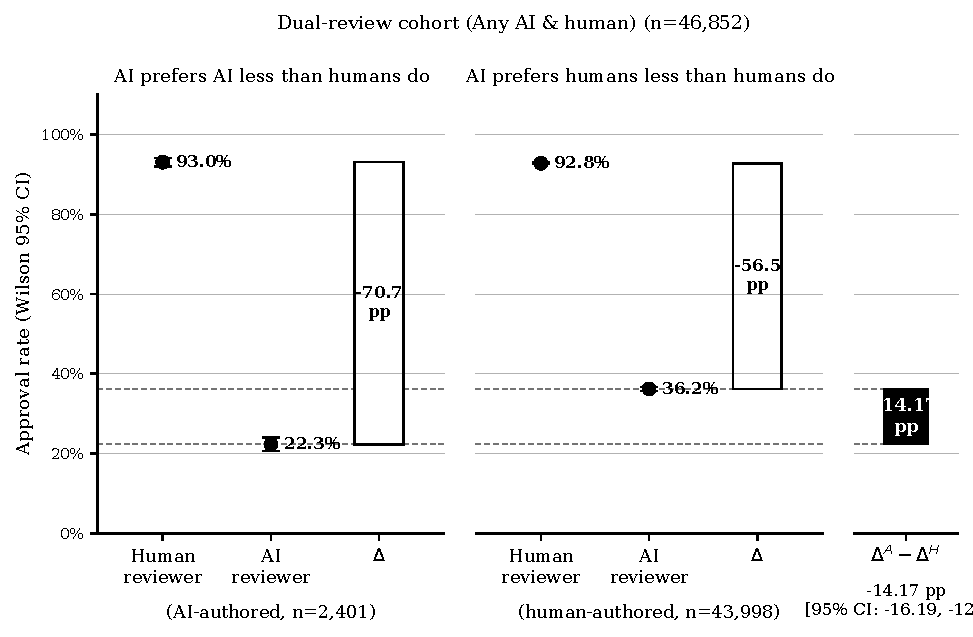
\includegraphics[width=\linewidth]{figures/figure2_withinpr.pdf}
    \caption{Within-PR AI-AI bias DiD on the \PLACEHOLDERDIDN{} PRs in the Dual-review cohort (Any AI \& human) --- AI bot reviewed \emph{and} human reviewed, with no commits between the AI's verdict and the human's review. Each panel holds author-type fixed and contrasts the human-reviewer and AI-reviewer approval rates (Wilson 95\% CIs); the labelled drop is the bracket entering $\widehat{\rbt^A - \rbt^H}$. \textbf{Left:} on AI-authored PRs, AI bots approve \PLACEHOLDERDIDB1{}~pp \emph{less} than humans do (``AI prefers AI less than humans do''). \textbf{Right:} on human-authored PRs, AI bots approve \PLACEHOLDERDIDB2{}~pp \emph{less} than humans do. The DiD is the difference of the two drops: $\widehat{\rbt^A - \rbt^H} = \PLACEHOLDERDIDPP{}$~pp (logit $\delta=\PLACEHOLDERDIDDELTA{}$, \PLACEHOLDERDIDPVAL{}). Both drops are negative because AI bots approve everything less than humans do; the drop on AI-authored PRs is \emph{more} negative, so the DiD is anti-self-preference.}
    \label{fig:withinpr}
\end{figure}

\begin{figure}[t]
    \centering
    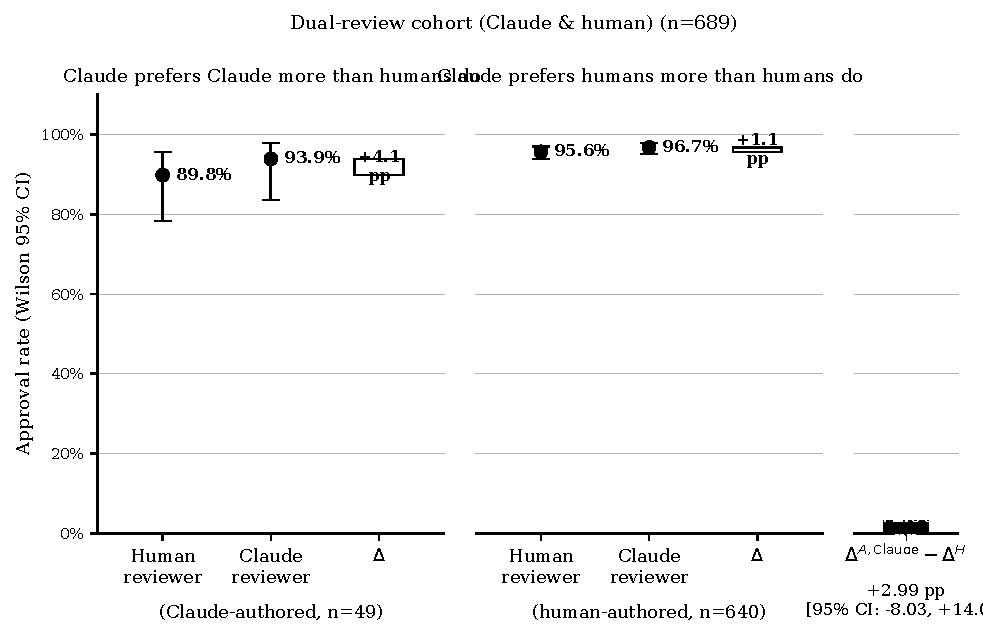
\includegraphics[width=\linewidth]{figures/figure2b_withinfamily_claude.pdf}
    \caption{Within-family check: Claude reviewers vs.\ human reviewers on Claude-authored vs.\ human-authored PRs, on the Dual-review cohort (Claude \& human) --- \PLACEHOLDERRQ3BCNFOR{} PRs (\PLACEHOLDERRQ3BCAUTHOR{} Claude-authored, \PLACEHOLDERRQ3BHAUTHOR{} human-authored). Same construction as Figure~\ref{fig:withinpr}: each panel holds author-type fixed and contrasts the human-reviewer and Claude-reviewer approval rates (Wilson 95\% CIs); the labelled drop is the within-author reviewer-type gap. \textbf{Left:} on Claude-authored PRs, Claude reviewers approve \PLACEHOLDERRQ3BCGAP{}~pp differently from humans. \textbf{Right:} on human-authored PRs, Claude reviewers approve \PLACEHOLDERRQ3BHGAP{}~pp differently from humans. The within-family DiD $\widehat{\rbt^{A,\text{Claude}} - \rbt^H}_\text{on Claude-auth} = \PLACEHOLDERRQ3BDIDPP{}$~pp (logit $\delta=\PLACEHOLDERRQ3BDIDDELTA{}$, \PLACEHOLDERRQ3BDIDPVAL{}) is direction-consistent with a small in-family preference but statistically indistinguishable from zero given the small Claude-authored cell.}
    \label{fig:withinfamily}
\end{figure}

\section{Call to action}
\label{sec:discuss}

Treat AI taste lock-in as a first-order empirical task, not a by-product of capability evaluation. Platforms (GitHub, Stack Overflow, npm, package registries) should publish monthly AI-activity reports. Model providers should include cross-family self-preference in post-training evaluations. Sectoral regulators should require the same for regulated agent markets. AI-mediated peer review~\citep{thakkar2025iclr} and social sycophancy~\citep{cheng2025elephant} indicate that AI can shape human judgments and behaviour---our pipeline lets such effects, if they emerge at scale, be \emph{tracked} rather than discovered retrospectively.

\paragraph{Future work: AI taste and the erosion of human taste.} Our pipeline measures \emph{whether} AI is the judge (RQ 2) and how its verdicts compare to humans' (RQ 3), but not whether sustained exposure to AI judgements erodes human taste itself --- the regime where uncertainty is over \emph{which goals to pursue at all}, and where thick-value alignment is required~\citep{edelman2025fullstack}. Before-and-after measurements of human research taste under controlled AI exposure on taste-dependent tasks, and tracking whether AI-first infrastructure~\citep{stein2026mcp} compounds the effect, are natural next steps.

\paragraph{Limitations.} (i)~\emph{Selection.} Our \PLACEHOLDERPRACTIVE{} repositories are critical OS software projects ranked by OpenSSF \texttt{criticality\_score}~\citep{ossf-criticality} (median stars \PLACEHOLDERSTARMED{}, see \Cref{app:repo-selection}). The criticality score favours load-bearing, multi-org, heavily-cross-referenced infrastructure rather than viral-popularity projects. We do not claim GitHub-wide representativeness.
(ii)~\emph{Detection false-negatives.} Heuristic detection cannot recover deliberately unattributed agent activity. Our verdict parser uses structural regex headers, not free-text sentiment.
(iii)~\emph{Sample size differs by RQ.} While RQ 1 uses all \PLACEHOLDERNPRS{} PRs, RQ 2 and RQ 3 condition on AI participation. For RQ 3 in particular, only \PLACEHOLDERDIDN{} PRs satisfy the within-PR DiD design (AI opinion + human explicit + no commits in between), of which \PLACEHOLDERDIDNAI{} are AI-authored.
(iv)~\emph{Correlational, not causal; identification rests on a homogeneity assumption.} Our evidence is observational. The DiD identification holds if PR quality shifts AI bot and human approval probabilities on the same scale --- a much weaker assumption than no-confounding, but not unconditional. Humans approve nearly all PRs they review (\PLACEHOLDERHAPPHRATE{} baseline) while AI bots have a much wider acceptance range, so the homogeneity assumption is the binding identification step. We address two potentially-violating mechanisms directly: anchoring (\Cref{app:anchoring} shows the human-side gap moves only \PLACEHOLDERANCHORADID{}~pp between cohorts with and without AI bot review present, ruling it out as the main driver) and authorship-classification error (silent AI use puts true-AI PRs in the human-author cell, attenuating the DiD toward zero --- if anything, this widens the true effect).
(v)~\emph{Merger attribution.} We measure reviews, not merges. No merges in our universe are attributed to AI bot accounts on our allowlist, but AI can still act \emph{through} a human merger when an AI approval gates the decision.
(vi)~\emph{Accelerators, not outcomes.} \emph{Accelerators} are observable, measurable patterns rather than disempowerment itself. They may also point in the opposite direction (e.g.\ switching costs can fall as well as rise).

\paragraph{Disclosure of AI usage.} AI assistants provided assistance with literature review, data analysis, and editing. The research idea, framework, and empirical approach are fully human-authored. Overall, the paper is primarily human-authored.

%%%%%%%%%%%%%%%%%%%%%%%%%%%%%%%%%%%%%%%%%%%%%%%%%%%%%%%%%%%%%%%%%%%%%%
\bibliography{references}
\bibliographystyle{icml2026}

%%%%%%%%%%%%%%%%%%%%%%%%%%%%%%%%%%%%%%%%%%%%%%%%%%%%%%%%%%%%%%%%%%%%%%
\newpage\appendix
\onecolumn
\section{Example pull requests}
\label{app:examples}
\input{appendix/examples.tex}

\section{Robustness and threats to validity}
\label{app:threats}
% Appendix B — robustness and threats to validity (expanded from §Limitations)

This appendix expands the limitations listed in the main paper.

\paragraph{B.1 Selection into the repository universe.}
We restrict to \PLACEHOLDERPRACTIVE{} critical OS software repositories ranked by OpenSSF \texttt{criticality\_score} (\Cref{app:repo-selection}). The resulting sample has median stars \PLACEHOLDERSTARMED{} (range \PLACEHOLDERSTARMIN{}--\PLACEHOLDERSTARMAX{}) and a criticality-score range of \PLACEHOLDERSCOREMIN{}--\PLACEHOLDERSCOREMAX{} --- it skews toward load-bearing, multi-org, heavily-cross-referenced open-source infrastructure (language toolchains, runtimes, foundation projects) rather than uniform popularity. Effects we estimate apply to ``critical OS software repositories''. We do not generalise to GitHub as a whole. In particular, chain-length growth in lower-criticality repositories may be smaller or larger than what we report, and we do not have data to say which.

\paragraph{B.2 Detection false-negatives: ``undercover'' agents.}
Our event-level detection (\S\ref{sec:methods}, \Cref{app:allowlist}) relies on two signals: bot-account logins, and \texttt{Co-Authored-By} trailers naming an AI tool. Commercial coding agents have been reported to include configuration options that suppress attribution in outward artefacts~---~e.g., an ``undercover mode'' reportedly present in at least one major coding agent's system prompt, revealed via a source-code leak in early 2026. PRs produced by such configurations appear as ordinary human activity to our detector. Consequently the measured AI-agent participation share in Figure~\ref{fig:headline} is a \emph{lower bound}. This does not overturn the paper's main claim (participation is growing) but tightens its interpretation: the true level is above what we measure, by an unknown amount.

\paragraph{B.3 Thin AI-approval slice in the within-PR test.}
Among our \PLACEHOLDERNREPOS{} repositories and \PLACEHOLDERNPRS{} PRs, only \PLACEHOLDERWITHINN{} carry an approving review from an AI bot, and only \PLACEHOLDERWITHINAIN{} of those are also AI-authored. This is not a sampling accident: fewer than ten bots in our allowlist ever emit an ``APPROVED'' review state, and only two (Cubic, CodeRabbit) do so routinely. The two-proportion $z$-test on the 24 vs.\ 137 cells has limited power. We report it as a null on explicit self-preference, with the understanding that larger-sample follow-ups are needed to distinguish a small positive effect from zero at the $\pm 5$~pp level.

\paragraph{B.4 Merger attribution: authors and reviewers, not mergers.}
We initially considered ``AI merger'' as a third dimension (author $\times$ reviewer $\times$ merger). No merges in our universe are attributed to AI bot accounts on our allowlist, so the merger dimension collapses to ``human'' on every observed PR. This is a substantive limitation: a human clicks the merge button on every merged PR in our window, but AI can still act \emph{through} that human---most obviously when an AI review's ``approved'' state is what gates a maintainer's decision to merge. Our observational design cannot separate a maintainer who merged \emph{because of} an AI approval from one who merged in spite of it. We also caution that our detector excludes merges performed under a maintainer's personal-access token by an AI app or merge-queue automation acting on their behalf. Such merges would appear as human in both the REST \texttt{merged\_by} field and the GraphQL timeline actor, and therefore cannot be recovered from the public event log alone.

\paragraph{B.5 Event timestamp ordering and chain definition.}
AI$\to$AI chains are defined on events sorted by timestamp within a PR. GitHub timestamps are accurate to seconds. Ties are broken by the API's default order (commit $<$ review $<$ review-comment $<$ issue-comment). Alternative tie-breaking does not change the head of the distribution meaningfully (mean and $p_{95}$ shift by $<$0.1 events). The tail (max chain = 13) is insensitive.

\paragraph{B.6 Reproducibility.}
Every number in the paper is derived from one of \texttt{data/pr\_events.parquet} (one row per actor/event) or \texttt{data/chains.parquet} (one row per PR, chain aggregates). These are produced by \texttt{scripts/03\_classify\_prs.py} and \texttt{05\_compute\_chains.py} respectively. The within-PR two-proportion test is produced by \texttt{scripts/06c\_within\_pr.py}. The upstream PR-event data (\texttt{data/prs/*.jsonl}) is collected by \texttt{scripts/02\_fetch\_prs.py} against the \PLACEHOLDERNREPOS{} repositories in \texttt{data/repos.json}, which itself is produced by \texttt{scripts/01\_build\_repo\_list.py} (\Cref{app:repo-selection} details this step). Given a valid GitHub token, the full pipeline reproduces the paper's numbers up to GitHub's own indexing non-determinism.


\section{Bot and AI-tool allowlists}
\label{app:allowlist}
\input{appendix/allowlist.tex}

\section{Repository-selection pipeline (replication)}
\label{app:repo-selection}
% Appendix --- Sample-selection pipeline

\paragraph{Overview.} The repository universe is selected via the OpenSSF
\emph{criticality\_score} \citep{ossf-criticality}.
The score is a published, replicable
ranking of GitHub projects by their structural importance to the open-source
ecosystem; using it directly addresses the well-known critique that
star-based selection over-weights short-lived viral projects relative to
load-bearing infrastructure
\citep{borges2018github, kalliamvakou2014promises, munaiah2017curating}.
We pin a published criticality snapshot, then filter and enrich it via the
GitHub REST API.

\paragraph{The OpenSSF criticality score.} For each project, the score is a
weighted arithmetic mean over normalised signals
\citep{ossf-criticality}. The signals used by the default \texttt{all.csv}
configuration are:
\begin{itemize}
\item \texttt{created\_since}: months since first commit;
\item \texttt{updated\_since}: months since last commit (negatively weighted);
\item \texttt{contributor\_count}: distinct authors over the project's history;
\item \texttt{org\_count}: distinct organisations among contributors;
\item \texttt{commit\_frequency}: average commits per week (last year);
\item \texttt{recent\_release\_count}: GitHub releases in the last year;
\item \texttt{updated\_issues\_count} and \texttt{closed\_issues\_count}: issues touched in the last 90 days;
\item \texttt{issue\_comment\_frequency}: comments per issue;
\item \texttt{github\_mention\_count}: cross-repo references (in commit messages and other repos' code).
\end{itemize}
The score lies in $(0, 1]$; higher is more critical. The OpenSSF
publishes a global score CSV to a public Google Cloud Storage bucket
(\texttt{gs://ossf-criticality-score/}) with a new snapshot every two
weeks. We pin a single snapshot (Step~1 below) so that re-running the
pipeline reproduces the same universe.

\paragraph{Step 1 --- Pin the criticality snapshot.} We use the
\PLACEHOLDERSNAPSHOT{} snapshot (\texttt{all.csv} variant, no deps.dev
dependent counts), which contains \PLACEHOLDERSNAPSHOTROWS{} scored
projects.

\paragraph{Step 2 --- Filter \& sort by score.} From the
\PLACEHOLDERSNAPSHOTROWS{} rows we keep those with a numeric
\texttt{default\_score} and a \texttt{repo.url} starting with
\texttt{https://github.com/}. After filtering: \PLACEHOLDERSCOREDROWS{}
rows. We sort descending by \texttt{default\_score}, breaking ties by
\texttt{repo.url} alphabetically for stability across reruns.

\paragraph{Step 3 --- Candidate cap (over-sample).} We take the top
\PLACEHOLDERCANDCAP{} candidates by score. The over-sample (vs.\ the
final \PLACEHOLDERFINALCAP{} target) absorbs drop-out in the next two
filtering steps: repos that no longer exist on GitHub, were renamed to a
private slug, or that are forks/archived/inactive.

\paragraph{Step 4 --- GitHub enrichment.} For each candidate we issue
\texttt{GET /repos/\{owner\}/\{name\}} (REST API, async, 8-way bounded
concurrency). The result populates the standard repo-metadata fields
(stars, forks, \texttt{pushed\_at}, license, default branch, etc.). HTTP
404 (deleted, renamed, or now-private) drops the row. After enrichment we
reject:
\begin{itemize}
\item \texttt{fork == true} (forks contribute no independent PR activity);
\item \texttt{archived == true};
\item \texttt{disabled == true};
\item \texttt{pushed\_at} strictly before \texttt{2025-04-01} (no
in-window PRs);
\item zero in-window PRs on GitHub (canonical development happens off GitHub --- LKML, git.apache.org, git.eclipse.org, etc.).
\end{itemize}

\paragraph{Step 5 --- Final cap.} Of the remaining \PLACEHOLDERPOSTACTIVITY{}, we keep the top
\PLACEHOLDERFINALCAP{} by criticality score as the final repo list.
Each row carries the GitHub-API fields plus the score, the within-snapshot
rank, the snapshot date, and the raw OpenSSF signal columns (so any
downstream re-weighting is possible without re-fetching the CSV).

\paragraph{Sample characteristics.}
\begin{itemize}
\item \PLACEHOLDERFINALCAP{} repositories selected from
\PLACEHOLDERSNAPSHOTROWS{} scored candidates $\to$ \PLACEHOLDERCANDCAP{}
top-by-score $\to$ \PLACEHOLDERENRICHOK{} successful GitHub enrichments
$\to$ \PLACEHOLDERPOSTACTIVITY{} after activity filter $\to$
\PLACEHOLDERFINALCAP{} after cap.
\item Criticality-score range: max \PLACEHOLDERSCOREMAX{}, min \PLACEHOLDERSCOREMIN{}.
\item Stars: min \PLACEHOLDERSTARMIN{}, median \PLACEHOLDERSTARMED{}, max \PLACEHOLDERSTARMAX{}.
\item Top languages: \PLACEHOLDERLANGTOP{}.
\end{itemize}

\paragraph{Analysed PRs.}
\begin{itemize}
\item Total PRs analysed: 3,109,979 (mean 311.0, median 93 per repo; p90 843, max 7,321).
\item Per-repo cap of \PLACEHOLDERPRSCAP{} PRs: 2 of \PLACEHOLDERFINALCAP{} repos (0.0\%) saturate the cap; for these the sampled rows are weighted toward the centre of the window by week-uniform subsampling rather than the most-recent months. All other repos have their full in-window PR history analysed.
\end{itemize}

\paragraph{Known selection biases.} The criticality score is itself an
opinionated metric: it favours older projects with multi-org contributor
bases, recent commit activity, frequent releases, and inbound cross-repo
references. Three biases inherited from this:
\begin{itemize}
\item Library-style projects score higher than application-style projects
of comparable importance because they accumulate inbound mentions from
their dependents' commit messages.
\item Pure-binary or assets-only repositories with no commits-as-history
(e.g.\ Wikipedia mirrors) are under-scored.
\item The score is computed over GitHub-visible signals only; non-GitHub
mirrors of important projects (e.g.\ many Apache and Eclipse Foundation
projects whose canonical home is elsewhere) are absent or under-counted.
\end{itemize}


\section{Supplementary figures}
\label{app:extra-figures}
\input{appendix/extra_figures.tex}

\section{Data and methods (full description)}
\label{app:methods}
% Appendix G — Data and methods, full description

\paragraph{Repository universe.} \PLACEHOLDERPRACTIVE{} critical OS software repositories selected by OpenSSF \texttt{criticality\_score}~\citep{ossf-criticality} (default\_score, snapshot \PLACEHOLDERSNAPSHOT{}), enriched via the GitHub REST API and filtered to drop forks, archived, disabled, and repos not pushed within the analysis window. Non-goal: GitHub-wide representativeness. Full selection procedure in \Cref{app:repo-selection}.

\paragraph{PR universe.} All PRs \emph{created} between 2025-04-01 and 2026-03-31 in those repositories (\PLACEHOLDERNPRS{} PRs), fetched via GitHub GraphQL with \texttt{orderBy:{CREATED\_AT,DESC}}. We record metadata, commits, reviews, review-thread comments, issue comments, and merge/close timeline events.

\paragraph{Event-level AI classification.} Adapting \citet{ghaleb2026fingerprinting}'s heuristics to event granularity, we classify each actor--event pair using two signals: the actor's GitHub login (matched against our 20-entry AI bot allowlist: \texttt{copilot-swe-agent[bot]}, \texttt{devin-ai-integration[bot]}, \texttt{cursor-agent}, \texttt{claude[bot]}, \texttt{coderabbitai}, \texttt{cubic-dev-ai}, \texttt{gemini-code-assist}, \texttt{copilot-pull-request-reviewer}, etc.\ -- see \Cref{app:allowlist}), and the event's payload text (commit message or PR body), scanned for a \texttt{Co-Authored-By} trailer naming an AI tool. We use a three-way taxonomy:
\begin{itemize}
\item \textbf{AI bot} --- actor login is on the AI bot allowlist.
\item \textbf{AI powered} --- actor login is human, but the payload carries an AI \texttt{Co-Authored-By} trailer.
\item \textbf{Human} --- neither of the above. This bucket may include silent AI support whose use was not declared via a trailer or bot login.
\end{itemize}
Pooled, AI bot $+$ AI powered events are referred to as \textbf{AI authored}. Handle/name mentions in free text (e.g.\ ``\texttt{@claude please fix}'') are \emph{not} treated as AI evidence: a human typing ``\texttt{@claude}'' in a comment is not themselves an AI contributor. Detected non-AI/maintenance bot events (Dependabot, Renovate, CI bots, etc.) are tracked separately and dropped from the AI-vs-human comparisons.

\paragraph{Chain length (RQ1).} Within a PR, order attributed events by timestamp. An \emph{AI$\to$AI chain} is a maximal contiguous subsequence of events with \texttt{actor\_type=AI bot}. AI powered events do not extend a chain --- chains track successive bot turns, not authorship attribution --- so this metric is a strict subset of AI authored. The per-PR metric is the longest such chain. We report the monthly share of PRs with chain $\geq$1, $\geq$2, $\geq$5.

\paragraph{AI verdict extraction.} AI bots issue native \texttt{APPROVED}/\texttt{CHANGES\_REQUESTED} review states on only \PLACEHOLDERAIOPRSNATIVE{} PRs in our window. The remaining ${\sim}70{,}000$ AI bot reviews carry the \texttt{COMMENTED} state but embed a structured verdict line that the bot itself writes in a stable template (e.g.,\ CodeRabbit's \texttt{Actionable comments posted: N}, Cubic's \texttt{N issues found}, Cursor Bugbot's \texttt{found N potential issues}, Sourcery's intro line). We extract verdicts via per-bot regex on these structured headers --- never on free-text sentiment. The full pattern catalogue and corpus-wide yield (\PLACEHOLDERAIOPPRS{} unique PRs with $\geq 1$ AI opinion after parsing, vs.\ \PLACEHOLDERAIOPRSNATIVE{} with native explicit votes only) is in \Cref{app:ai-verdict-regex}. Gemini Code Assist reviews are free-prose without a stable structured header and are left unclassified.

\paragraph{AI vs.\ human judge counters (RQ2).} Unlike the RQ3 DiD, which pools native and regex-parsed AI verdicts on the Dual-review cohort (Any AI \& human), the RQ2 ``explicit AI review'' and ``AI-only review'' monthly shares count native \texttt{APPROVED}/\texttt{CHANGES\_REQUESTED} review states only and impose no commit-ordering constraint between the AI and human reviews, so they are a strict native-only lower bound on AI's share as judge.

\paragraph{Baseline approval rates.} As a reference point: across all PRs, human-authored PRs are approved (merged with $\geq 1$ approving review) at 50.0\% ($n$=2,606,804), versus 37.3\% for AI-authored PRs ($n$=81,341).

\paragraph{Within-PR AI-AI bias DiD (RQ 3).} For each PR we assign \texttt{author\_type}~$\in\{$AI authored, human$\}$. ``AI authored'' here is the rolled-up category --- it covers both AI bot author logins and human-author commits/PR bodies that carry an AI co-author trailer (i.e.\ AI powered). Commits authored after the PR was opened are excluded so review-cycle AI activity does not retroactively mark the original PR as AI authored. The DiD universe is the \emph{Dual-review cohort (Any AI \& human)}: PRs that received both an AI bot opinion (native or parsed) AND a human explicit review, with no commits pushed strictly between the AI's first opinion timestamp and the human's first explicit-review timestamp (so both reviewers evaluated the same commit graph). We compute the four reviewer-type $\times$ author-type cells with Wilson 95\% CIs and fit a logistic regression with HC0 standard errors on the long-format dataset \texttt{Pr(approve) $\sim$ author\_AI + reviewer\_AI + author\_AI:reviewer\_AI}; the interaction coefficient is the DiD estimate. Anchoring is tested as a robustness check by stratifying on whether an AI bot has reviewed (\Cref{app:anchoring}).

\paragraph{Within-PR within-family DiD (RQ 3, Claude check).} The pooled DiD treats all AI bots as one ``AI'' reviewer cell. To test whether \emph{Claude-based} reviewers prefer Claude-authored code more than humans do, we re-run the same logit-DiD framework on the \emph{Dual-review cohort (Claude \& human)}: PRs with a Claude opinion AND a human explicit review (with the same no-commits-between filter as the pooled cohort); authors restricted to Claude vs human; Claude reviewer approves vs human reviewer approves. ``Claude opinion'' for this analysis combines native \texttt{APPROVED}/\texttt{CHANGES\_REQUESTED} states with regex-parsed verdict-line headers from Claude's review bodies and PR-thread \texttt{issue\_comment}s (\texttt{**Recommendation**: Approve}, \texttt{**Recommendation**: Request changes}, etc. --- \Cref{app:ai-verdict-regex}). Hand-audit precision on the parsed reject pattern is 122/122 = 100\% across the corpus, with zero false positives in a 37,506-comment scan of non-Claude logins.

\paragraph{Scope: authors and reviewers, not mergers.} We measure AI participation through authoring and reviewing, not merging. No merges in our universe are attributed to AI bot accounts on our allowlist, so ``AI merger'' is not an informative dimension in this window. We discuss the limitations of that framing---including the fact that AI can still act \emph{through} a human merger---in §\ref{sec:focus}.


\section{AI bot verdict regex catalogue}
\label{app:ai-verdict-regex}
% Appendix F — AI bot verdict regex catalogue
% Companion to RQ3 / Figure 2. Documents the per-bot regex used to extract
% approve/reject verdicts from the structured-format headers each bot writes
% in its `COMMENTED` review bodies.

AI bots issue native \texttt{APPROVED}/\texttt{CHANGES\_REQUESTED} review states on only \PLACEHOLDERAIOPRSNATIVE{} PRs in our window. The remaining ${\sim}70{,}000$ AI bot reviews carry the \texttt{COMMENTED} state but embed a structured verdict line that the bot itself writes in a stable template. We extract verdicts via per-bot regex on these structured headers; we do \emph{not} run sentiment classification on free-text.

\paragraph{Pattern catalogue (per bot, first match wins).} Each pattern targets a fixed structured header that the bot writes in a stable template. Only AI bots on the existing allowlist are scanned. Cursor's no-bugs verdict requires a leading green-check emoji; trailing-LGTM matches for Claude require an ``addressed/resolved'' phrase about prior feedback. \texttt{<details>...</details>} blocks are stripped before matching for Claude bodies to prevent the trailing-LGTM regex hitting quoted text inside the ``Extended reasoning'' appendix.

\begin{table*}[t]
\centering\footnotesize
\caption{AI bot verdict regex catalogue. Yields are corpus-wide event counts; each row is one bot $\times$ verdict combination.}
\label{tab:ai-verdict-regex}
\begin{tabular}{@{}llp{0.42\linewidth}r@{}}
\toprule
Bot & Verdict & Regex (pattern shape) & Yield \\
\midrule
Cubic & approve & \texttt{**No issues found** across N file(s)} & 2,462 \\
Cubic & reject  & \texttt{**N issues found** across N file(s)} ($N\geq 1$) & 1,313 \\
CodeRabbit & approve & \texttt{**Actionable comments posted: 0**} & 4,491 \\
CodeRabbit & reject  & \texttt{**Actionable comments posted: N**} ($N\geq 1$) & 12,888 \\
Copilot PR Reviewer & approve & \texttt{Copilot reviewed \dots and generated no new comments} & 1,099 \\
Copilot PR Reviewer & reject  & \texttt{Copilot reviewed \dots and generated N comments} ($N\geq 1$) & 18,267 \\
Greptile & approve & \texttt{<sub>N files reviewed, no comments</sub>} & 306 \\
Greptile & reject  & \texttt{<sub>N files reviewed, M comments</sub>} ($M\geq 1$) & 720 \\
Cursor Bugbot & approve & \texttt{✅ Bugbot reviewed your changes and found no bugs!} & 55 \\
Cursor Bugbot & reject  & \texttt{Cursor Bugbot \dots found N potential issues} ($N\geq 1$) & 1,504 \\
Sourcery & approve & \texttt{Hey [there|@user] - I've reviewed \dots and they look great} & 986 \\
Sourcery & reject  & \texttt{Hey [there|@user] - I've \{found N | left some | here's some feedback\}} & 1,635 \\
Claude & approve (start) & \texttt{LGTM\dots} anchored to absolute start of body & 717 \\
Claude & approve (trailing) & \texttt{\dots prior \{feedback|concerns|issues\} addressed --- LGTM.} & 16 \\
Gemini Code Assist & --- & free-prose; no stable structured header, left unclassified & 0 \\
\bottomrule
\end{tabular}
\end{table*}

\paragraph{Coverage (\% of each bot's COMMENTED reviews classified).} Cubic 100\%, CodeRabbit 86\%, Cursor Bugbot 79\%, Sourcery 79\%, Copilot PR Reviewer 57\%, Greptile 54\%, Claude 69\% (the rest are \texttt{\#\# Claude Code Review} setup messages, correctly excluded as no-opinion), Gemini Code Assist 0\% (free-prose only). Aggregate over all AI bot \texttt{COMMENTED} reviews: 13.3\% parsed-approve, 48.4\% parsed-reject, 37.6\% unmatched (mostly Gemini and non-template Copilot prose reviews, left unclassified).


\section{Robustness: does AI's review anchor humans?}
\label{app:anchoring}
\input{appendix/anchoring_robustness.tex}

\end{document}
